%%%% imav.tex
% This is the tex-file for the IMAV 2014 conference
% for questions / remarks / bugs regarding the files, please contact info@imavs.org
% You can use this style for your conference, as long as you refer to the IMAV 2014
% in a comment similar to this one.
% Of course, the IMAV 2014 is not liable for any aspects of its use.

\documentclass[letterpaper]{article}
% The style file
\usepackage{imav}
% Use the postscript times font!
\usepackage{times}
\usepackage{graphicx}
\usepackage{float}
\usepackage{array}
\usepackage{tabularx}
\usepackage{booktabs} 
\usepackage{url} 
\usepackage{caption}
%\usepackage{algorithm} % Install algorithm support and uncomment if needed
%\usepackage{algorithmic} % Install algorithmc support and uncomment if needed
\usepackage{wasysym}
%\numberwithin{algorithm}{chapter}
%\usepackage{algorithmicx}
% the following package is optional:
%\usepackage{latexsym}

\title{Comparative Analysis of Cameras for ArUco Marker Recognition in Unmanned Aerial Vehicles}
\author{Souza, J. V. N. \thanks{Email address: vitorjo8gbi@gmail.com}, Sobrinho Junior, D. F. \thanks{Email address: durvaljunior117@gmail.com}, Santos, L. G.\thanks{Email address: leandro.santos@ifbaiano.edu.br}, Oliveira, R. G. \thanks{Email address: rafaelgomesdeoliveiraa@gmail.com}, Afonso, S. P. \thanks{Email address: saviopessoaafonso@gmail.com}, \\ Souza, J. M. \thanks{Email address: jeovanamiranda218@gmail.com}, Costa, G. S. N. \thanks{Email address: gustavosncosta@gmail.com}, Lima, F. S. \thanks{Email address: fabio.lima@ifbaiano.edu.br} and. Cotrim, R. M. \thanks{Email address: reinaldo.cotrim@ifbaiano.edu.br} \\ Instituto Federal de Educação, Ciência e Tecnologia Baiano - Campus Guanambi, Guanambi, Bahia}

\begin{document}

\maketitle
\thispagestyle{empty} % Keep this to remove page number from first page

\begin{abstract}
Remotely Piloted Aircraft Systems (RPAS), commonly known as drones, have been integrated into various activities since the first decade of the 21st century, driven by technological advancements and globalization \cite{silva2017steam}. However, the high cost of drones, particularly due to the image capture device, limits their accessibility in social and educational sectors, with the imaging component representing up to half of the total equipment cost. To address this challenge, this research evaluates the effectiveness of four affordable cameras — IMX519, IPCAM, ESP32, and ANALOGIC — that were not originally designed for drones, aiming to identify their potential in detecting two-dimensional ArUco markers. The analysis considers several criteria, including resolution, power consumption, brightness, weight, and detection performance. The tests were conducted outdoors, with the cameras configured to capture images at five flight altitudes (3, 6, 9, 12, and 15 meters) under varying light conditions throughout the day. ArUco markers of different sizes (100, 200, 300, and 400 mm) were used to assess the cameras' detection capabilities. The results revealed significant variations in performance among the cameras. The IPCAM stood out with the best overall detection average, consistently demonstrating superior performance, particularly at lower altitudes and with 400 mm markers. Although the ESP32 offers advantages in power consumption, weight, and cost, these differences are secondary compared to the IPCAM's remarkable superiority in marker detection. Therefore, the results indicate that the IPCAM is the most recommended choice for efficient ArUco marker detection, offering the best balance between performance and cost-effectiveness for RPAS applications with computer vision systems.
\end{abstract}
% ------ START INTRODUCTION -------------
\section{Introduction} \label{section:introduction}
The so-called Remotely Piloted Aircraft Systems (RPAS), popularly known as “drones”, are devices that have become intrinsically linked to various industrial, operational, social and leisure activities since the first decade of the 21st century. These technological transformations driven by globalization require individuals to adapt to the contemporary world \cite{silva2017steam}. %(SILVA, et al, 2017).

However, there are still several challenges that prevent the integration of these innovations into the daily lives of society, within low-capital corporations, and in education, particularly due to their high cost.

One of the factors contributing to their elevated price is the image and video capture device, which is essential for several tasks, such as area mapping, object detection, precision agriculture, and inspections. However, in many cases, this device can represent up to half of the total equipment cost. Thus, there is a need for the development or functional repurposing of photography and filming technologies aimed at increasing the accessibility of RPAS.

From this perspective, this research proposes a functional redirection by comparing the effectiveness of four affordable camera models, which, although not originally developed for use in drones, are evaluated in this context to identify their potential application in such devices. The different cameras were tested with the detection of two-dimensional ArUco markers of different sizes, considering variables such as light levels (LUX) and flight altitude, elements that are capable of influencing the system's performance.

According to the analysis of the results obtained, it is possible to identify which environmental conditions and camera combinations offer the best accuracy in detecting ArUco markers and, consequently, determine the device with the greatest cost-benefit for use in RPAS with embedded computer vision systems.
%Remotely Piloted Aircraft Systems (RPAS), popularly known as “drones”, are devices that have become intrinsically linked to various industrial, operational, social and leisure activities since the first decade of the 21st century. These technological transformations driven by globalization require individuals to adapt to the contemporary world (SILVA, et al, 2017).

%The constant transformations in society driven by globalization demand that individuals adapt to the new technologies present in the contemporary world \cite{silva2017steam}. Drones, vehicles that do not require a crew on board, are part of these new technologies and are widely represented across various sectors of society.

%Due to the importance of these vehicles, several educational institutions have started to incorporate drones into their curricula and to promote participation in related student competitions that encompass the use of MAVs. These initiatives aim of developing in students the technical skills required in the job market, as well as enhance research expertise for the preparation of scientific work among them.

%Over time, the use of cameras in UAVs (Unmanned Aerial Vehicles) has become essential to increase the precision and capacity to carry out tasks that require capturing images and recording videos. In addition, advanced tools like computer vision can be used to extract relevant data from the images acquired and process them for subsequent procedures, further expanding the potential of drones in various fields.

%However, the high cost of acquiring quality equipment, especially cameras, represents a significant financial challenge, as these devices are essential for various tasks such as mapping areas, detecting objects, precision agriculture, and inspections. In light of this challenge, it is crucial to develop efficient approaches to evaluate the financial investment and electrical consumption associated with obtaining these devices.

%In this context, this study aims to provide technical and practical information to assist students in choosing cameras available on the market that align with purchasing power of their institutions, supplying the technological quality required to recognize two-dimensional ArUco-type markers.
%----------------END INTRODUCTION-------------

% --------------- STARTS RELATED WORKS -------------
\section{Related Works}
ArUco markers are fiducial squares with a black-and-white binary pattern, widely used for pose estimation in several applications, including autonomous robots, virtual trainers, and unmanned aerial vehicles \cite{Bacik2017} \cite{Yang2018} \cite{hansen2024active}. The OpenCV library, used for developing computer vision algorithms, has a module dedicated to the detection of these markers \cite{Romero-Ramirez2019}. %(Romero-Ramirez et al., 2019)

ArUco markers are configured in a 7x7 matrix, totaling 49 cells, with 24 allocated to the border and 25 to the data area. This area is subdivided into 15 cells to ensure integrity and 10 for information encoding, allowing for up to 1,024 combinations. Integrity is ensured through a logical verification scheme across the columns, enhancing the robustness of the detection system \cite{silva2014evaluation}. %(Silva, Tommaselli & Artero, 2014)

Despite the choice of the ArUco marker, other binary square fiducial markers, such as Matrix \cite{rekimoto1998matrix} and ARTag \cite{fiala2010designing}, also have similar applications. When detected by cameras, these markers enable the execution of a single pre-established function in the UAV, while also allowing the estimation of the position of a monocular camera at minimal cost, with high robustness and speed.

In a literature review on autonomous vehicles using RGB camera-based vision, \cite{pavel2022vision} highlighted the effectiveness of these cameras under different visibility conditions and in complex scenarios. Studies such as those by \cite{borowczyk2017autonomous}, \cite{Munoz-Salinas2017}, and  \cite{hu2019sinet} demonstrated that the use of monocular cameras, combined with deep learning, overcame the limitations of other sensors such as LiDAR, especially in detecting objects at different scales, under various lighting conditions, and across different viewing angles and speeds, enabling precise mapping, localization, positioning, and landing of the aircraft.

\cite{Yang2018} conducted a study that combined two cameras with distinct characteristics — a fisheye lens camera and a stereoscopic camera — with the objective of facilitating the autonomous landing of drones on mobile ground vehicles in GPS-denied environments. This work is closely related to the present study, as the features of different cameras and their adaptability to various lighting conditions are critical factors for both accurate detection and precise drone control.

A recent study by \cite{Sarmadi2021}, which utilized an event-based camera for ArUco marker detection, revealed that this type of sensor achieves a significantly higher detection rate under high-speed conditions and varying levels of illumination compared to conventional RGB cameras. Key variables such as flight altitude, lighting conditions, and rapid camera movement were found to influence detection efficiency, highlighting the importance of considering these factors when assessing the performance of different drone-mounted cameras in ArUco marker detection.

% -------------END RELATED WORKS ---------------

% --------- START MATERIALS AND METHODS --------
\section{Materials and Methods}
This study was carried out in the Drone and Prototyping Laboratory of the Centro de Estudos Tecnológicos em Informática e Agronomia (CETEIA, Center for Technological Studies in Informatics and Agronomy, in English) at the Instituto Federal de Educação, Ciência e Tecnologia Baiano — Guanambi Campus, in Brazil.
%This study was carried out in the drone and prototyping laboratory of the Centro de Estudos Tecnológicos em Informática e Agronomia (CETEIA, Center for Technological Studies in Agronomy and Informatics, in English) of the Federal Institute of Education, Science and Technology Baiano --- Guanambi Campus, in Brazil.

Initially, image capture devices were selected based on availability and a maximum configuration cost of \$150.00, including the device and the equipment required for its full operation. Based on these criteria, four different configurations were designated for standardization purposes as IMX519, IPCAM, ESP32, and ANALOGIC.

To perform the comparative analysis, the different systems were tested with the detection of standardized ArUco two-dimensional markers in sizes of 100, 200, 300, and 400 mm using the 'Original ArUco' dictionary, although for the purposes of this analysis, only ID48 was used

Detections were performed in an open-air environment, on the surface of a road built with concrete blocks. ArUco markers of various sizes were arranged side by side for image capture. The four camera configurations were mounted on the RPA to ensure that all images were captured under the same conditions.

Flights were set at altitudes of 3, 6, 9, 12, and 15 meters, and for each established flight altitude, the cameras were configured to capture 30 images, excluding those where one or more of the four marker sizes were out of frame. The collection resulted in a total of 90 images per flight altitude for each camera. Thus, each camera produced 450 images, totaling 1,800 images in the dataset

Since the images were captured outdoors at different times throughout the day, ambient light levels were also measured, as lighting is a determining factor in the quality of the image recorded by the camera sensor. The light was measured using the INS-1381 Digital Luxmeter during each flight conducted for image capture. The luxmeter was leveled in a horizontal position on a pedestal 120 cm above the ground and positioned less than 2 meters from the ArUco markers. Additionally, image metadata, such as longitude, latitude, and time, were recorded.




%This study was carried out in the drone and prototyping laboratory of the Center for Technological Studies in Agronomy and Informatics (CETEIA or CTSAI in English) of the Federal Institute of Education, Science and Technology Baiano --- Guanambi Campus, in Brazil.

%Four Setups consisting of different models of image capture devices were analyzed: Setup 1 (microcomputer Raspberry with IMX519 camera); Setup 2 (Wanscam HW0043 IP security camera); Setup 3 (ESP32-CAM microcontroller); and Setup 4 (Foxeer Monster V2 analog FPV system). More detailed specifications of these sensors will be presented below.

%In order to carry out a comparative analysis between the four different Setups, with a view to identifying two-dimensional ArUco markers in real time, five flight heights were defined (3; 6; 9; 12, and 15 meters), and four sizes of ArUco marker (10x10; 20x20; 30x30; 40x40 centimeters). 

%The ArUco markers were placed side by side to capture the images in an open environment, under the surface of a road made of concrete blocks. The images were captured in good light conditions, between 10 am and 4 pm. 

%The four Setups were loaded onto the drone so that during the capture, the images were subjected to the same lighting conditions since this factor can interfere with the identification of the ArUco marker. For each of the flight heights defined, the cameras were configured to capture a set of 10 images.


\subsection{Setups}
\subsubsection{Setup 1: IMX519}

Configuration 1 utilizes the IMX519 digital image capture sensor, which provides 16 megapixels (Mp) and supports a maximum resolution of 4656 x 3496 pixels, with a transfer rate of up to 9 frames per second (fps) at this resolution. At lower resolutions, the sensor can achieve up to 120 fps. However, for the purposes of this study, a resolution of 1920 x 1080 pixels at 30 fps was selected. 

\begin{figure}[H]
\centering
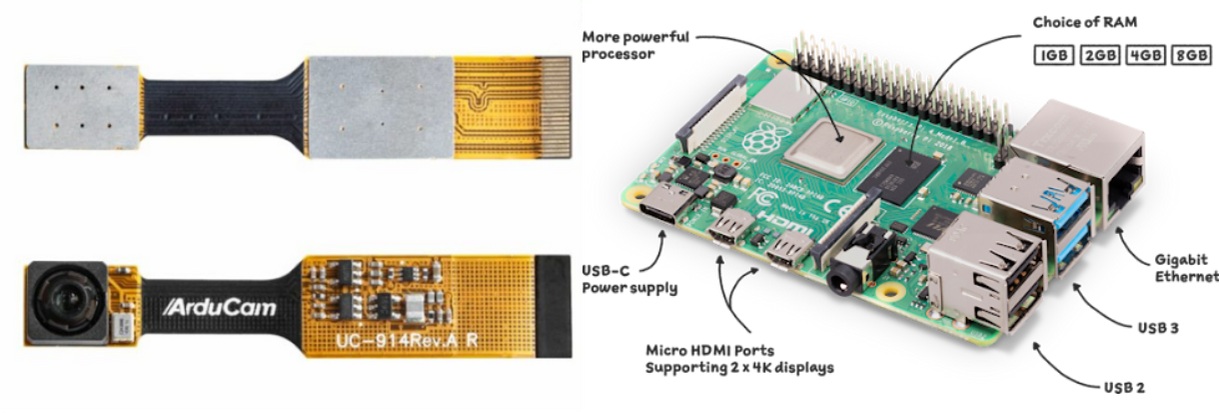
\includegraphics[width=0.8\columnwidth]{images/setup_1.png}
\caption{IMX519 camera module and Raspberry Pi 4B that make up the setup 1}
\label{figure:setup_1}
\end{figure}

It also features an 80° (diagonal) field of view, a 1/2.53-inch CMOS sensor, an f/1.75 lens, dimensions of 34 mm x 34 mm x 26.23 mm, a weight of 4g, and operates within a temperature range of 0ºC to 70ºC with an operating voltage of 5 volts.

For its operation, the Raspberry Pi 4 Model B single-board computer was utilized, connected via a flat cable to the Camera Serial Interface (CSI). According to the datasheet released by \cite{raspberrypi4datasheet}, this model is equipped with a high-performance 64-bit quad-core processor, offering robust performance and thus enabling the efficient execution of complex tasks.

\subsubsection{Setup 2: IPCAM}
Configuration 2 consists of the Hw0043 image capture device, a security camera with 1 MP and a maximum resolution of 1280 x 720 pixels, which was the resolution used. It supports an image transfer rate of up to 30 fps and can be connected via Ethernet port or WiFi.

\begin{figure}[H]
\centering
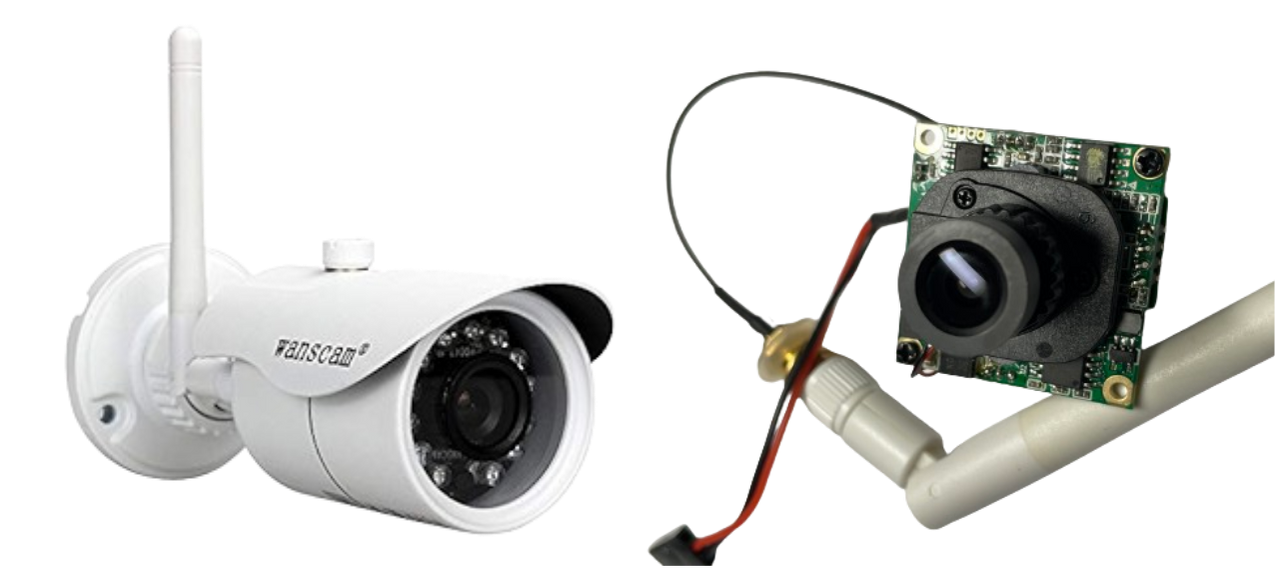
\includegraphics[width=0.6\columnwidth]{images/setup_2.png}
\caption{Wanscam HW0043 Wi-Fi security camera}
\label{figure:setup_2}
\end{figure}

The device operates in a temperature range of -10ºC to 50ºC, features a 110º diagonal field of view (FOV), a 1/4” CMOS sensor, a 3.6 mm lens, and operates at a voltage of 5V. To reduce its weight, the protective aluminum casing was removed; therefore, the camera now weighs approximately 31g and measures 32.3 mm x 32.8 mm x 38.9 mm. This camera is integrated with the MT7601un WiFi module, which operates in accordance with the IEEE 802.11b standard and can achieve speeds of up to 150 Mbps.


\subsubsection{Setup 3: ESP32}
Configuration 3 is composed of the OV2640 IoT image capture device, manufactured by OmniVision. It features a 2-megapixel sensor, a maximum resolution of 1600x1200 pixels, and an image transfer rate of up to 60 fps. However, a resolution of 1024x768 pixels was utilized for this study. The device includes a 1/4-inch CMOS sensor, dimensions of 8.1 mm x 8.1 mm x 5.7 mm, and operates within a temperature range of 0ºC to 50ºC, with a voltage requirement of 5V.

\begin{figure}[H]
\centering
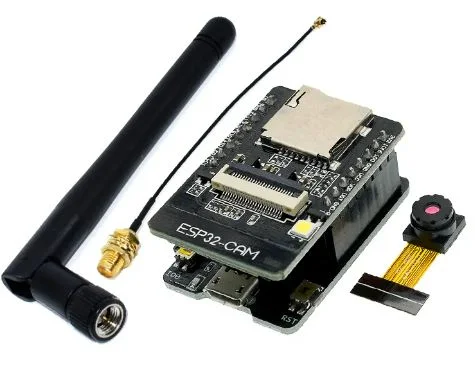
\includegraphics[width=0.6\columnwidth]{images/setup_3.png}
\caption{OV2640 62º Camera}
\label{figure:setup_3}
\end{figure}

Using a small flat cable, the OV2640 camera is integrated into the ESP32-CAM board, which includes a serial input compatible with the device. This assembly weighs 10 grams, with a lens that has a 62º field of view (FOV), operates at 5V, and exhibits a power consumption ranging between 160 mA and 310 mA during operation.

\subsubsection{Setup 4: ANALOGIC}
\begin{figure}[H]
\centering
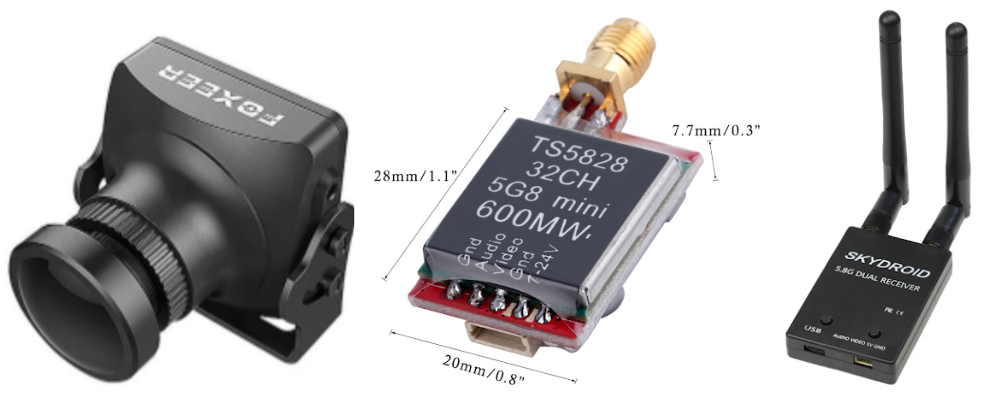
\includegraphics[width=0.6\columnwidth]{images/setup_4.png}
\caption{Foxeer camera, video transmitter and receiver that make up the setup 4}
\label{figure:setup_4}
\end{figure}

The Foxeer Monster V2 camera is the only analog device tested. It offers a resolution of 1280 x 960, with a 1/2.9-inch CMOS sensor and a 3.6 mm lens. Its operating voltage is 5V, and it functions within a temperature range of -10ºC to 50ºC. Unlike the others, the Foxeer Monster V2 has 1200 TVL (Television Lines). To operate this camera, it is necessary to integrate a video transmitter system into the aircraft, specifically using the TS5828 model with 32 channels and 600 mW. The ground station, on the other hand, utilized a Skydroid UVC 5.8 video receiver, connected to a computer via a USB port. The camera has dimensions of 28 mm x 26 mm x 30 mm and, together with the video transmitter, weighs 19 grams.

\subsection{RPA Specifications}

The aircraft used for this study was built on a Tarot 650 frame, configured as a quadcopter multirotor with a carbon fiber structure. It was equipped with 30A Blheli Oneshot-125 LittleBee Electronic Speed Controllers (ESCs) and Sunnysky 3508-600 KV brushless motors. Additionally, a PixHawk 1 (3DR) flight controller, configured with Arducopter firmware, was utilized to maintain the control and stability of the aircraft, enabling automated flights.

A GPS module integrated with a compass was used to determine latitude and longitude, allowing for precise identification of the quadcopter's orientation. Similarly, to accurately measure the drone's altitude, the Benewake TFmini Plus module, equipped with a laser distance sensor, was employed, providing measurements up to 6 meters with an error margin of ±5 cm.



\subsection{Measuring electrical consumption}

The electrical consumption tests of the four setups were carried out on a bench, using the Riden DC6012 source, which provides instantaneous data on voltage, current, power, and consumption of the equipment connected to it.

\subsection{ArUco marker recognition}

The objective of the ArUco marker recognition test is to determine how the distance between markers and ambient lighting affects each camera setup, thereby analyzing each setup's ability to identify reference points of varying sizes.

\begin{figure}[H]
\centering
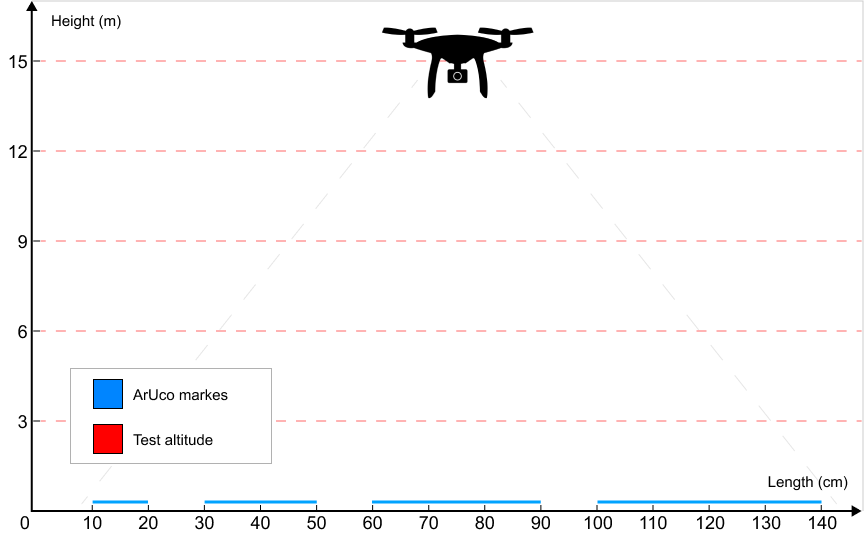
\includegraphics[width=1\columnwidth]{sky_drone_graphic.png}
\caption{Representative illustration of the positioning of arUco markers during flights to capture images at different heights.}
\label{figure:sky_drone_graphic}
\end{figure}

According to \cite{dalianis2018evaluation}, system evaluations can be qualitative or quantitative. Qualitative evaluation involves obtaining feedback from users about their satisfaction with the system, while quantitative evaluation objectively measures system performance and is often applied in detection and classification algorithms. \cite{powers2008evaluation} highlights the confusion matrix as an essential tool for evaluating binary classification, allowing the observation of correct and incorrect predictions, categorized as True Positive (TP), False Negative (FN), False Positive (FP), and True Negative (TN). \cite{varoquaux2023evaluating} and \cite{markoulidakis2021multiclass} illustrate the importance of this matrix for calculating evaluation metrics, where Precision = TP / (TP + FP) represents the proportion of correctly classified positives, and Accuracy = (TP + TN) / (TP + FN + FP + TN) reflects the overall proportion of correctly classified instances.

Therefore, the values of each image were classified into a confusion matrix to analyze how these variables affect detection based on precision and accuracy metrics.

\subsection{Algorithm}

TTo optimize the testing process and obtain more accurate data, software was developed that directly communicates with the drone and the selected cameras. This software automates drone control and ArUco detection, in addition to saving the processed images. This enables a precise evaluation of the performance of the image capture devices used, significantly reducing the time and effort required compared to manual methods.

The development of this software was carried out using the object-oriented programming language Python, version 3.10.9. Two libraries were essential for automating the tests: Pymavlink, version 2.4.41, which manages drone communication and control via the MAVLink protocol, and OpenCV, version 4.9.0.80, which facilitates communication with the cameras and ArUco detection through digital image processing.

The code employs the object-oriented paradigm, creating classes that encapsulate behavior and preserve their internal state through attributes and methods. A specific class was developed for each logical or physical component of the test. For example, the 'Drone' class communicates directly with the physical drone and controls it through its methods. Each camera was also abstracted as a class.

The Abstract Factory design pattern was used to create classes for each camera, using inheritance to maintain their common characteristics and polymorphism to expose differing behaviors. These approaches ensure that the existing code does not need to be modified, following the Open-Closed and Dependency Inversion principles. This ensures modular and maintainable code, facilitating the addition of new devices and functionalities in the future

\begin{figure}[H]
\centering
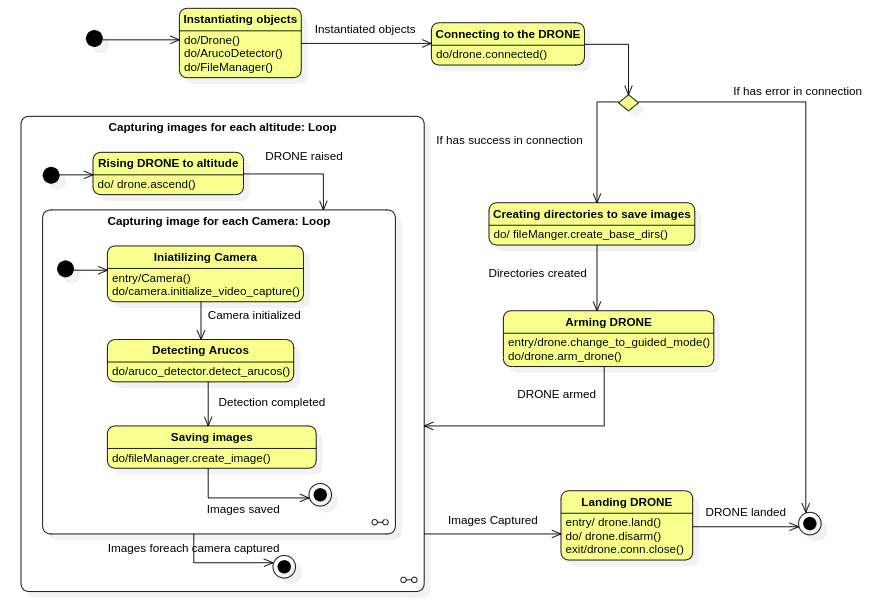
\includegraphics[width=1\columnwidth]{state_machine_diagram.png}
\caption{State machine diagram illustrating the algorithm's states during testing}
\label{figure:state_machine_diagram}
\end{figure}

In the state machine diagram shown in Figure \ref{figure:state_machine_diagram}, the software states during the execution of the tests can be observed. The process begins with the instantiation of the objects necessary to perform the tasks, followed by an attempt to connect to the drone via telemetry. If the connection is not established, the code is terminated. If the connection is successful, directories are created to save the images captured during the test.

Next, the drone’s flight mode is set to GUIDED, where the drone is controlled by commands sent by an operator or software, rather than following a pre-programmed flight plan or being manually controlled, and then its motors are armed. For each altitude defined in the test, the drone ascends and detects the ArUcos in all configured cameras. After completing the entire process, the drone switches to LAND mode and lands, finally closing the connection between the software and the drone.

%\subsection{Tables}
%When inserting a table, you can choose the appropriate style - Table~\ref{table:results} below is an example. Put the caption under the table.

%\begin{table}[hbt]
%\begin{center}
%\begin{tabular}{|l|c|c|c|c|}
%\hline
%& IMX519 & Wanscam HW0043 & OV2640 IoT & Foxeer Monster V2\\
%\hline
%Max. Resolution (Pixels) & 3280 x 2464 & 1280 x 720 & 1600 x 1200 & 1280 x 960\\
%CMOS size (Inch) & 1/2.53 & 1/4 & 1/4 & 1/2,9\\
%Diagonal Field of View (DFOV) & 78º & 110º & 62º & -\\
%Power supply (Volts) & 5 & 5 & 5 & 5\\
%\hline
%\end{tabular}
%\caption{Information about each camera.}
%\label{table:results}
%\end{center}
%\end{table}

%\section{Math and Units}

%\subsection{Math}
%Include equations in Latex with the equation environment:

%\begin{equation} \label{equation:n}
%n = \sqrt{\frac{a}{b}}
%\end{equation}

%If used inside the text, use the \$-sign: $a = b-c$. Only do this for short formulas.

%\subsection{Units}
%Always use SI units first, possibly adding other units in parentheses.

%\section{Referencing}

%\subsection{In-document referencing}
%Always introduce a figure as 'Figure X', as in "Figure \ref{figure:imav2022_logo} shows the IMAV logo.", or "The IMAV logor is shown in Figure \ref{figure:imav2022_logo}." Subsequently, the word 'figure' can be used. The same goes for tables ('Table \ref{table:results}'). Equations do not have to be introduced this way. If they are referenced to, 'Equation \ref{equation:n}' should be used. Sections are referred to as 'Section \ref{section:introduction}'\footnote{Footnotes are placed like this.}

%\subsection{Referencing to literature}
% Citations are numbered consecutively with square brackets \cite{DEWAGTER2014} - this is determined by the bibliography style `unsrt'. The references can be described in bibtex format in a separate bib-file (see the bibliography statement close to the end of the tex-file).  The sentence punctuation follows the brackets \cite{NOLFIPOWLIM}. Multiple references \cite{DEWAGTER2014,NOLFIPOWLIM} are each numbered with separate brackets or in sequence as \cite{DEWAGTER2014,NOLFIPOWLIM,BISHOP2006}.
%Follow the reference style at the end of this document. Papers that have not been published should be cited as "unpublished". Papers that have been submitted for publication should be cited as "submitted for publication". Papers that have been accepted for publication, but not yet specified for an issue should be cited as "to appear". Capitalize only the first word in a paper title, except for proper nouns and element symbols.
%Below, \cite{DEWAGTER2014} is a reference to a conference paper, \cite{NOLFIPOWLIM} to a journal paper, and \cite{BISHOP2006} to a book.

%\section{Publishing Policy}
%The IMAV proceedings will only be distributed in digital form. The submitting author is responsible for obtaining agreement of all his / her coauthors and any consent required from sponsors before submitting a paper. The authors are obliged to cite relevant prior work.

\section{Results and Discussions}

Table \ref{table:specifications_and_consumption} presents the data on electrical consumption and weight of the configurations evaluated in this study. The electrical consumption and weight of the camera directly impact flight autonomy and are, therefore, critical factors to be considered when defining the drone configuration.

\begin{table}[H]
\begin{center}
\resizebox{\columnwidth}{!}{
\begin{tabular}{c m{3cm} c c c c c}
\toprule
Setup & \centering CAM & V (V) & C (Ah) & W (g) & COST (US\$) \\
\toprule
1 & \centering IMX519 + Raspberry PI 4B. & 5.0 & 0.40 & 50 & 144.00 \\
\midrule
2 & \centering Wanscam Hw0043 + Wifi MT7601UN. & 5.0 & 0.20 & 31 & 25.00 \\
\midrule
3 & \centering OV2640 IOT + ESP32-Cam. & 5.0 & 0.16 & 10 & 6.00 \\
\midrule
4 & \centering Foxeer Monster V2 + TS5828. & 12.0 & 0.45 & 19 & 60.00 \\
\bottomrule
\end{tabular}}
\caption{Specifications and consumption of the setups studied}
\label{table:specifications_and_consumption}
\captionsetup{font=footnotesize,skip=0pt}
\caption*{CAM = camera, V = voltage (V), C = current (Ah), W = weight (g).}
\end{center}
\end{table}


Configuration 1 has the heaviest weight (50 g) and relatively high power consumption (0.40 Ah) compared to the others. The combination of its weight and power consumption results in a significant reduction in the drone's flight time relative to the other configurations. Configuration 2, weighing 31 g and consuming 0.20 Ah, offers a good balance between weight and power consumption, which results in greater flight autonomy compared to configurations 1 and 4.

Configuration 3 is the lightest (10 g) and has the lowest power consumption (0.16 Ah), providing the drone with greater autonomy than the other configurations. Configuration 4 has an intermediate weight (19 g) but the highest power consumption (0.45 Ah), leading to reduced flight autonomy.

The analysis of the cameras' performance in detecting ArUco markers reveals that accuracy, a metric used for evaluating classifiers, is influenced by both the marker size and the camera's altitude, as shown in Figure \ref{figure:cameras_accuracy}.

\begin{figure}[H]
\centering
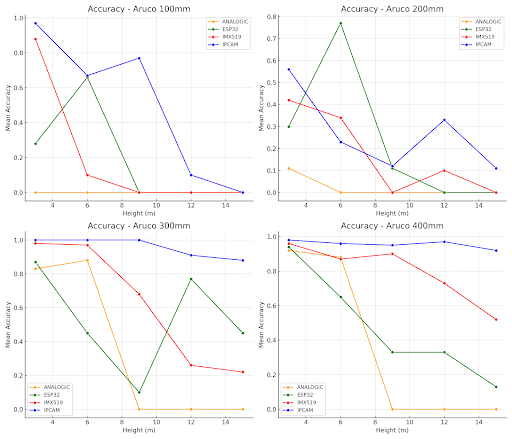
\includegraphics[width=1\columnwidth]{images/cameras_accuracy.png}
\caption{Accuracy of the studied cameras in detecting ArUco markers of different sizes and flight altitudes}
\label{figure:cameras_accuracy}
\end{figure}

The camera analyses revealed marked differences in their performance depending on the variables tested. The ANALOGIC camera had the lowest accuracy rate among the options evaluated. This camera showed an accuracy rate of almost zero for 100 mm and 200 mm ArUcos at all tested altitudes, indicating significant difficulty in identifying these markers at different heights. However, for 300 mm and 400 mm ArUcos, the ANALOGIC demonstrated better performance at altitudes ranging from 3 to 9 meters. Despite this, its performance dropped drastically above these altitudes, evidencing a limitation in the ability to maintain accuracy at greater distances.

The ESP32 demonstrated a superior ability to handle larger markers, such as 300 mm and 400 mm, even at higher altitudes. This suggests that the ESP32 has good resolution and sensitivity to identify large markers at greater distances. However, the camera consistently performed poorly in detecting smaller ArUcos (100 mm and 200 mm), regardless of altitude. Still, compared to the IMX519, the ESP32 was more effective at lower altitudes for small markers. However, as altitude increased, the IMX519 proved to be more suitable, especially for 300 mm and 400 mm markers, with a higher accuracy rate at greater heights.

The IMX519 showed intermediate performance, but its effectiveness increased with altitude and marker size. It also excelled, especially at higher altitudes with large markers, demonstrating a superior ability to maintain accuracy under these conditions. This suggests that the camera is more adaptable to variations in altitude and marker size, offering a good solution for scenarios where marker height and size are greater.

Finally, the IPCAM achieved the highest accuracy rates among all the cameras tested and proved to be the most stable. The IPCAM maintained a high level of consistent performance across different altitudes and ArUco sizes, making it the most reliable choice for practical applications.

Initially, for the 100 mm ArUco marker, a decrease in detection accuracy is observed as altitude increases. The IPCAM maintains an accuracy of 0.68 up to 6 meters, but the graph indicates a sharp decline from 9 meters onward, reaching nearly zero at 12 meters. Despite this, the IPCAM still outperforms the other cameras. The IMX519 showed a detection accuracy of 0.89 only at 3 meters, drastically reducing to near zero at 6 meters, and above this height, detection is null. The ESP32, however, demonstrates an accuracy of 0.30 at 3 meters and reduces to zero from 9 meters, thus maintaining low accuracy from the lowest height. The ANALOGIC camera exhibits the worst performance, with null detections at all altitudes.

\begin{figure}[H]
\centering
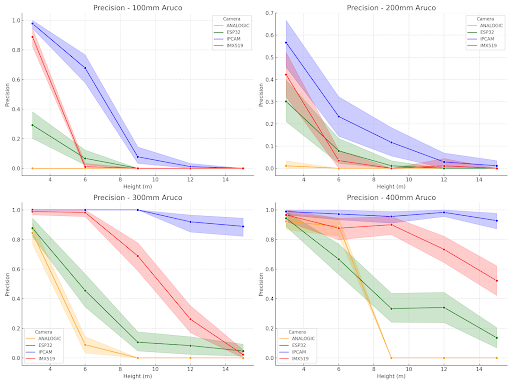
\includegraphics[width=1\columnwidth]{images/accuracy_detecting_aruco.png}
\caption{Precision in detecting ArUco markers at different altitudes and sizes for the various studied cameras}
\label{figure:accuracy_detecting_aruco}
\end{figure}

When increasing the size of the ArUco marker to 200 mm, the detection accuracy of the ANALOGIC camera remained the poorest performer, with zero detections at all flight altitudes. However, the IPCAM and IMX519 cameras achieved precisions of 0.57 and 0.42, respectively, in detecting the marker at a 3 m altitude, dropping drastically to zero from 9 m onwards. The ANALOGIC camera recorded the lowest precision at all altitudes for this marker size (200 mm). Similarly unsatisfactory, the ESP32 presented a maximum precision of 0.30 at a 3 m altitude, with a sharp decline at 6 m. For this marker size, at altitudes above 6 m, all cameras exhibited poor performance, with precision practically reduced to zero.

Furthermore, for the 300 mm ArUco marker, all cameras demonstrated significant improvement in performance, with precision greater than 0.84 at a 3 m altitude. For this marker size, the IPCAM stood out by maintaining accuracy above 0.88 even at an altitude of 15 m. The IMX519 camera maintained accuracy around 0.98 up to 6 m, decreasing to 0.69 at 9 m. The ESP32 camera achieved the highest accuracy (0.87) at a 3 m altitude, but this dropped sharply to 0.11 at 9 m. As for the ANALOGIC camera, despite achieving an accuracy of 0.84 at 3 m, it failed to detect the marker from 9 m onwards.

Finally, with the 400 mm ArUco marker, the detection rate was the highest across all cameras. The IPCAM camera achieved accuracy above 0.92 even at the highest altitude. Similarly, the IMX519 camera also performed well, maintaining accuracy above 0.73 at a height of 12 m. The ESP32 camera achieved accuracies of 0.94 and 0.67 at heights of 3 and 6 m, respectively, but its performance decreased to 0.33 at heights above 9 m. The ANALOGIC camera, despite achieving accuracies of 0.92 and 0.89 at 3 and 6 m, respectively, did not detect any markers at heights above 9 m, even though it was evaluating the largest marker size in this study.

Figure \ref{figure:true_positive_rate} illustrates the relationship between the True Positive Rate (TPR) and luminosity (in LUX) for different ArUco marker sizes (100 mm, 200 mm, 300 mm, and 400 mm) and various camera types (ANALOGIC, ESP32, IMX519, IPCAM). The TPR is a metric that indicates the proportion of markers correctly identified by the camera relative to the total number of markers present. Consequently, the graph enables a comparative analysis of the cameras' performance under varying lighting conditions and for different marker sizes.

For the 100 mm ArUco markers, all cameras show relatively low TPR rates, especially under low-light conditions. As luminosity increases, performance improves slightly, but detection remains limited for all cameras. Some variations are observed, with the IPCAM and IMX519 cameras achieving slightly higher rates in environments with luminosity levels above 100,000 LUX, although rates remain generally low.

\begin{figure}[H]
\centering
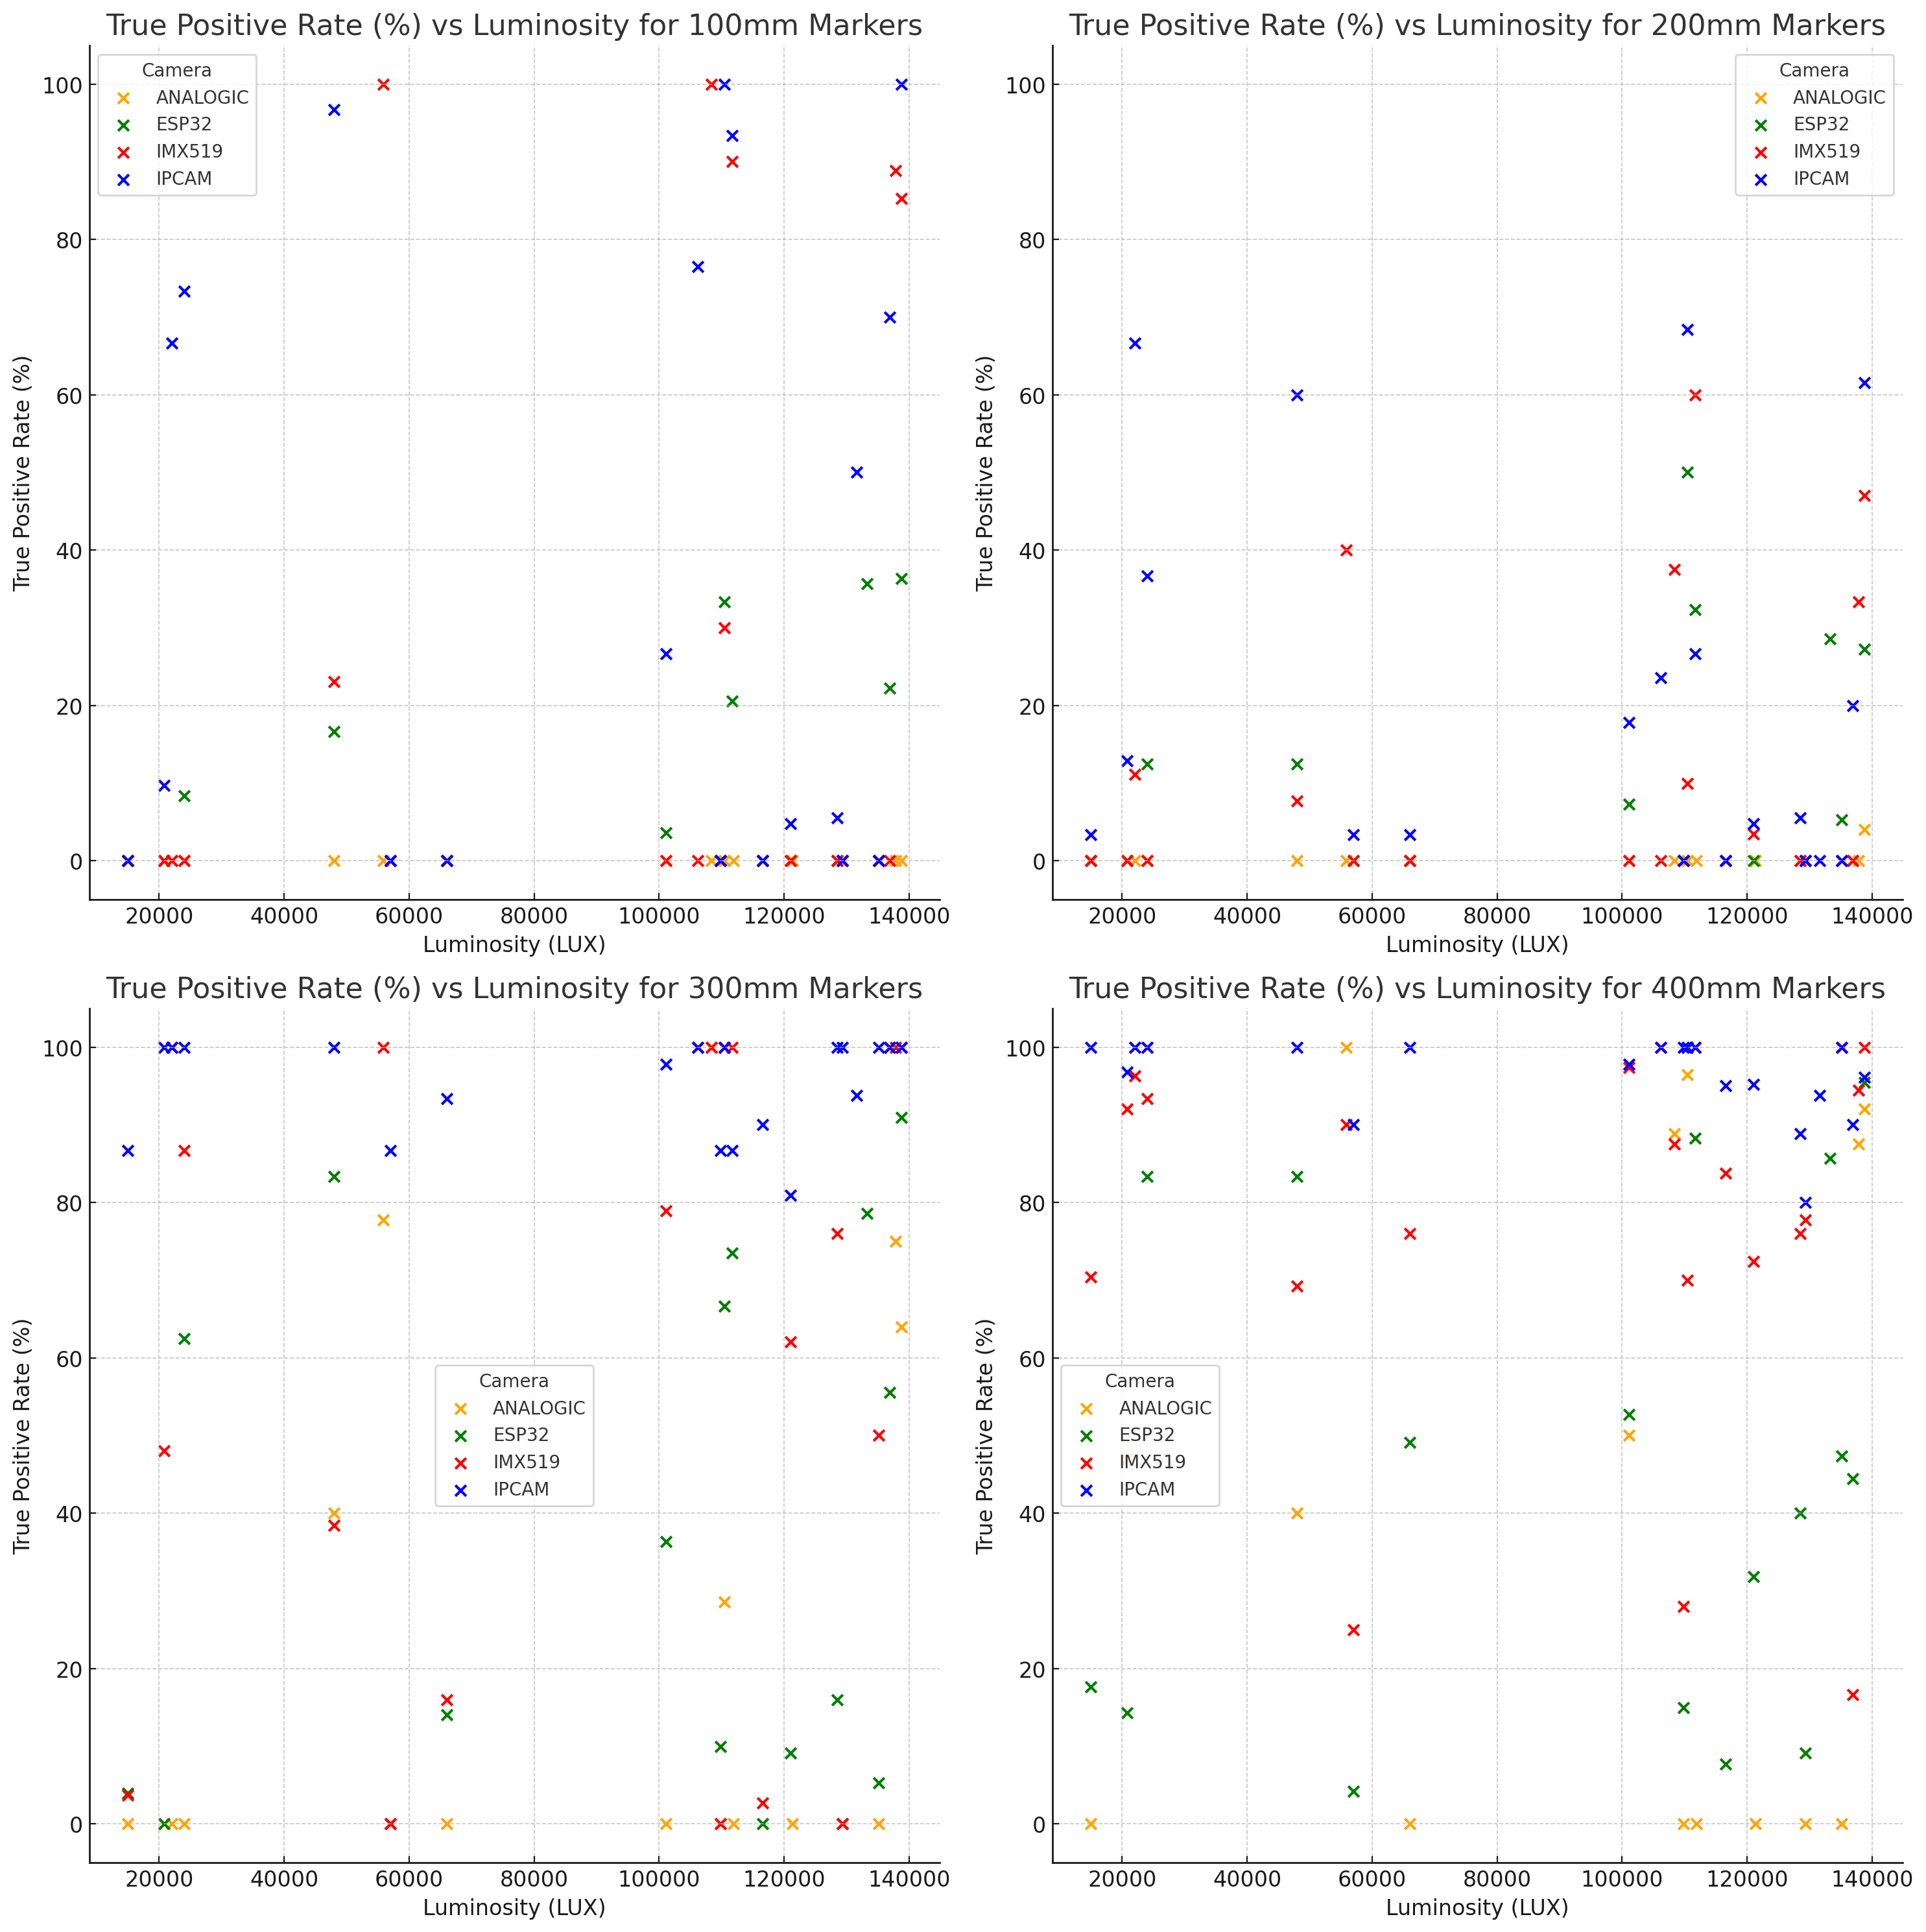
\includegraphics[width=0.8\columnwidth]{images/true_positive_rate2.png}
\caption{True positive rate in the detection of ArUco markers of different sizes by the cameras studied as a function of brightness.}
\label{figure:true_positive_rate}
\end{figure}
In the case of the 200 mm markers, there is a similar behavior, where TPR rates remain low under low light conditions. As the light intensity increases, especially above 100,000 LUX, the IMX519 and IPCAM cameras begin to exhibit better performance, with higher TPR compared with the other cameras. The ESP32, however, consistently shows low performance under all lighting conditions.

When analyzing the 300 mm markers, an overall improvement in camera performance is observed. TPR rates increase significantly, especially for the IMX519 and IPCAM cameras, which exceed 80\% under high light conditions. The ANALOGIC camera also demonstrates reasonable performance, while the ESP32 continues to show lower TPR rates, indicating less efficient performance in detecting these markers.

For 400 mm markers, the IMX519 and IPCAM cameras achieve even higher TPR rates, often close to 100\%, under high luminosity conditions. The ANALOGIC camera also maintains solid performance in this scenario. However, the ESP32 shows lower TPR rates compared to the other cameras, even with greater luminosity and larger markers.


\section{Conclusion}
Using the collected data, the relationship between the detection of ArUco markers, observation height, and marker dimensions was analyzed. Generally, the larger the ArUco marker, the higher the detection rate. Conversely, increasing the distance between the camera and the marker causes a significant drop in detection efficiency. Additionally, lighting has proven to be an important factor, with greater light intensity substantially enhancing camera performance, allowing for more accurate identification of the markers.

In this study, the IPCAM camera demonstrated the best overall performance in detecting ArUco markers, particularly at low altitudes and with 400 mm markers. Moreover, it showed significant superiority over the other cameras in detecting smaller markers. When considering other variables, such as power consumption, weight, and acquisition cost, the ESP32 camera exhibited superior performance in all these aspects. However, the differences in these criteria are minimal and do not have a significant impact compared to the more substantial difference in detection performance between the cameras, which clearly favors the IPCAM.

Thus, the results suggest that, among the cameras studied, the IPCAM emerged as the most suitable choice for detecting ArUco markers. These findings were crucial in guiding the Drones Guanambi team in selecting the camera to be used in the indoor and outdoor events of IMAV 2024.

The IMX519 camera, because it needs the Raspberry, is the heaviest and has the second highest power consumption. The Wanscam, on the other hand, had the second lowest power consumption and the highest detection rate of ArUco markers.

When comparing the two cameras, it is crucial to consider other factors. The IMX519 requires connection to a microcomputer, increasing energy consumption, and the need to monitor the status of the microcomputer to ensure correct data transfer. In contrast, the Wanscam Hw0043 Camera offers a simpler connection and data transfer, consumes less energy, and is more affordable.

The IMX519 camera has a higher resolution, reaching up to 16 MP (megapixels). This can be advantageous for teams with more programming experience, allowing programmatic adjustments to the camera's quality and focus, potentially improving the detection of ArUcos.

The choice between the Wanscam Hw0043 Camera and the IMX519 will depend on the specific needs of the project. The Wanscam Hw0043 is a robust and economical choice for intermediate altitudes, while the IMX519, with its high resolution and potential for programmatic adjustments, can offer significant advantages for projects that demand superior image quality and greater technical flexibility, even if it has higher electrical consumption and financial costs.



%\section*{Acknowledgements}
%Here you can place your acknowledgment.

% BIBLIOGRAPHY:
 %use {unsrt}:
\bibliographystyle{unsrt}
\bibliography{imav_bibliography}

% The following lines are necessary for showing the appendices correctly, do not change!
%\appendix
%\newcommand{\appsection}[1]{\let\oldthesection\thesection
%  \renewcommand{\thesection}{Appendix \oldthesection:}
%  \section{#1}\let\thesection\oldthesection}
% appendices are now indicated by appsection:

%\appsection{Data}
%If appendices are necessary, they appear at the end of the document. Use `appsection' instead of `section'.
%\appsection{More data}
%Even more data.
\end{document}

